\documentclass[twoside]{book}

% Packages required by doxygen
\usepackage{fixltx2e}
\usepackage{calc}
\usepackage{doxygen}
\usepackage[export]{adjustbox} % also loads graphicx
\usepackage{graphicx}
\usepackage[utf8]{inputenc}
\usepackage{makeidx}
\usepackage{multicol}
\usepackage{multirow}
\PassOptionsToPackage{warn}{textcomp}
\usepackage{textcomp}
\usepackage[nointegrals]{wasysym}
\usepackage[table]{xcolor}

% Font selection
\usepackage[T1]{fontenc}
\usepackage[scaled=.90]{helvet}
\usepackage{courier}
\usepackage{amssymb}
\usepackage{sectsty}
\renewcommand{\familydefault}{\sfdefault}
\allsectionsfont{%
  \fontseries{bc}\selectfont%
  \color{darkgray}%
}
\renewcommand{\DoxyLabelFont}{%
  \fontseries{bc}\selectfont%
  \color{darkgray}%
}
\newcommand{\+}{\discretionary{\mbox{\scriptsize$\hookleftarrow$}}{}{}}

% Page & text layout
\usepackage{geometry}
\geometry{%
  a4paper,%
  top=2.5cm,%
  bottom=2.5cm,%
  left=2.5cm,%
  right=2.5cm%
}
\tolerance=750
\hfuzz=15pt
\hbadness=750
\setlength{\emergencystretch}{15pt}
\setlength{\parindent}{0cm}
\setlength{\parskip}{3ex plus 2ex minus 2ex}
\makeatletter
\renewcommand{\paragraph}{%
  \@startsection{paragraph}{4}{0ex}{-1.0ex}{1.0ex}{%
    \normalfont\normalsize\bfseries\SS@parafont%
  }%
}
\renewcommand{\subparagraph}{%
  \@startsection{subparagraph}{5}{0ex}{-1.0ex}{1.0ex}{%
    \normalfont\normalsize\bfseries\SS@subparafont%
  }%
}
\makeatother

% Headers & footers
\usepackage{fancyhdr}
\pagestyle{fancyplain}
\fancyhead[LE]{\fancyplain{}{\bfseries\thepage}}
\fancyhead[CE]{\fancyplain{}{}}
\fancyhead[RE]{\fancyplain{}{\bfseries\leftmark}}
\fancyhead[LO]{\fancyplain{}{\bfseries\rightmark}}
\fancyhead[CO]{\fancyplain{}{}}
\fancyhead[RO]{\fancyplain{}{\bfseries\thepage}}
\fancyfoot[LE]{\fancyplain{}{}}
\fancyfoot[CE]{\fancyplain{}{}}
\fancyfoot[RE]{\fancyplain{}{\bfseries\scriptsize Generated by Doxygen }}
\fancyfoot[LO]{\fancyplain{}{\bfseries\scriptsize Generated by Doxygen }}
\fancyfoot[CO]{\fancyplain{}{}}
\fancyfoot[RO]{\fancyplain{}{}}
\renewcommand{\footrulewidth}{0.4pt}
\renewcommand{\chaptermark}[1]{%
  \markboth{#1}{}%
}
\renewcommand{\sectionmark}[1]{%
  \markright{\thesection\ #1}%
}

% Indices & bibliography
\usepackage{natbib}
\usepackage[titles]{tocloft}
\setcounter{tocdepth}{3}
\setcounter{secnumdepth}{5}
\makeindex

% Hyperlinks (required, but should be loaded last)
\usepackage{ifpdf}
\ifpdf
  \usepackage[pdftex,pagebackref=true]{hyperref}
\else
  \usepackage[ps2pdf,pagebackref=true]{hyperref}
\fi
\hypersetup{%
  colorlinks=true,%
  linkcolor=blue,%
  citecolor=blue,%
  unicode%
}

% Custom commands
\newcommand{\clearemptydoublepage}{%
  \newpage{\pagestyle{empty}\cleardoublepage}%
}

\usepackage{caption}
\captionsetup{labelsep=space,justification=centering,font={bf},singlelinecheck=off,skip=4pt,position=top}

%===== C O N T E N T S =====

\begin{document}

% Titlepage & ToC
\hypersetup{pageanchor=false,
             bookmarksnumbered=true,
             pdfencoding=unicode
            }
\pagenumbering{alph}
\begin{titlepage}
\vspace*{7cm}
\begin{center}%
{\Large My Project }\\
\vspace*{1cm}
{\large Generated by Doxygen 1.8.13}\\
\end{center}
\end{titlepage}
\clearemptydoublepage
\pagenumbering{roman}
\tableofcontents
\clearemptydoublepage
\pagenumbering{arabic}
\hypersetup{pageanchor=true}

%--- Begin generated contents ---
\chapter{Class Index}
\section{Class List}
Here are the classes, structs, unions and interfaces with brief descriptions\+:\begin{DoxyCompactList}
\item\contentsline{section}{\hyperlink{structcell}{cell} \\*The structure for a header block }{\pageref{structcell}}{}
\item\contentsline{section}{\hyperlink{structMemory}{Memory} \\*The structure of the \hyperlink{structMemory}{Memory} }{\pageref{structMemory}}{}
\end{DoxyCompactList}

\chapter{File Index}
\section{File List}
Here is a list of all documented files with brief descriptions\+:\begin{DoxyCompactList}
\item\contentsline{section}{utils/\hyperlink{ipcTools_8c}{ipc\+Tools.\+c} \\*This file helps to manage icp Semaphores and mutex }{\pageref{ipcTools_8c}}{}
\item\contentsline{section}{utils/{\bfseries ipc\+Tools.\+h} }{\pageref{ipcTools_8h}}{}
\item\contentsline{section}{utils/\hyperlink{memory_8c}{memory.\+c} \\*This file is the .c that allow to do all the operations of allocation/free on the memory }{\pageref{memory_8c}}{}
\item\contentsline{section}{utils/{\bfseries memory.\+h} }{\pageref{memory_8h}}{}
\item\contentsline{section}{utils/\hyperlink{structures_8c}{structures.\+c} \\*This file is the .c used to manipulate the header block }{\pageref{structures_8c}}{}
\item\contentsline{section}{utils/{\bfseries structures.\+h} }{\pageref{structures_8h}}{}
\end{DoxyCompactList}

\chapter{Class Documentation}
\hypertarget{structDataRibbon}{}\section{Data\+Ribbon Struct Reference}
\label{structDataRibbon}\index{Data\+Ribbon@{Data\+Ribbon}}


The structure for the Data Ribbon.  




{\ttfamily \#include $<$structures.\+h$>$}

\subsection*{Public Attributes}
\begin{DoxyCompactItemize}
\item 
\mbox{\Hypertarget{structDataRibbon_a73207b4f107779b04d8657658b734495}\label{structDataRibbon_a73207b4f107779b04d8657658b734495}} 
int \hyperlink{structDataRibbon_a73207b4f107779b04d8657658b734495}{size}
\begin{DoxyCompactList}\small\item\em size of the array that contains data \end{DoxyCompactList}\item 
\mbox{\Hypertarget{structDataRibbon_a18fadaaa4662125922b4c432245adf3b}\label{structDataRibbon_a18fadaaa4662125922b4c432245adf3b}} 
int \hyperlink{structDataRibbon_a18fadaaa4662125922b4c432245adf3b}{used\+Size}
\begin{DoxyCompactList}\small\item\em size used of the array \end{DoxyCompactList}\item 
\mbox{\Hypertarget{structDataRibbon_a1e46999166f48122a974d11fc1d00f4c}\label{structDataRibbon_a1e46999166f48122a974d11fc1d00f4c}} 
void $\ast$$\ast$ \hyperlink{structDataRibbon_a1e46999166f48122a974d11fc1d00f4c}{ribbon}
\begin{DoxyCompactList}\small\item\em array that contains the data \end{DoxyCompactList}\item 
\mbox{\Hypertarget{structDataRibbon_a76e03f2eb05be8f3cf963183ae6a5b9e}\label{structDataRibbon_a76e03f2eb05be8f3cf963183ae6a5b9e}} 
int $\ast$ \hyperlink{structDataRibbon_a76e03f2eb05be8f3cf963183ae6a5b9e}{allocated\+Map}
\begin{DoxyCompactList}\small\item\em Array that say if an element of the ribbon is allocated (1) or not(0) \end{DoxyCompactList}\end{DoxyCompactItemize}


\subsection{Detailed Description}
The structure for the Data Ribbon. 

The documentation for this struct was generated from the following file\+:\begin{DoxyCompactItemize}
\item 
utils/structures.\+h\end{DoxyCompactItemize}

\hypertarget{structMemory}{}\section{Memory Struct Reference}
\label{structMemory}\index{Memory@{Memory}}


The structure of the \hyperlink{structMemory}{Memory}.  




{\ttfamily \#include $<$memory.\+h$>$}



Collaboration diagram for Memory\+:
\nopagebreak
\begin{figure}[H]
\begin{center}
\leavevmode
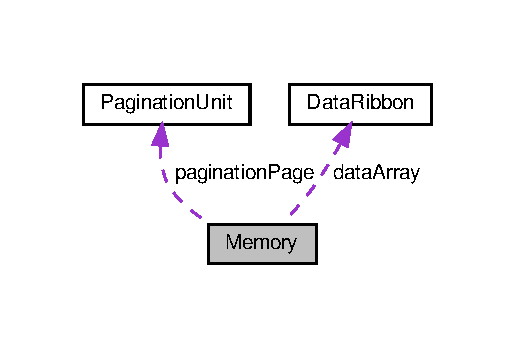
\includegraphics[width=162pt]{structMemory__coll__graph}
\end{center}
\end{figure}
\subsection*{Public Attributes}
\begin{DoxyCompactItemize}
\item 
\mbox{\Hypertarget{structMemory_a168856d0599e2430a961979a4ca204d0}\label{structMemory_a168856d0599e2430a961979a4ca204d0}} 
int \hyperlink{structMemory_a168856d0599e2430a961979a4ca204d0}{total\+Size}
\begin{DoxyCompactList}\small\item\em The total size of the memory. \end{DoxyCompactList}\item 
\mbox{\Hypertarget{structMemory_a719ceb2b6e7f494de7673fc5bacc02f8}\label{structMemory_a719ceb2b6e7f494de7673fc5bacc02f8}} 
int \hyperlink{structMemory_a719ceb2b6e7f494de7673fc5bacc02f8}{used\+Size}
\begin{DoxyCompactList}\small\item\em The used size of the memory. \end{DoxyCompactList}\item 
\mbox{\Hypertarget{structMemory_a9dd2c85715ec465afbefc0ce63c2cde8}\label{structMemory_a9dd2c85715ec465afbefc0ce63c2cde8}} 
int \hyperlink{structMemory_a9dd2c85715ec465afbefc0ce63c2cde8}{mutex}
\begin{DoxyCompactList}\small\item\em The mutex of the memory, to guarantee the unicity of the access to the memory. \end{DoxyCompactList}\item 
\mbox{\Hypertarget{structMemory_aecc2163eec0b2330f6e8ce789c5be7e7}\label{structMemory_aecc2163eec0b2330f6e8ce789c5be7e7}} 
\hyperlink{structcell}{Header} \hyperlink{structMemory_aecc2163eec0b2330f6e8ce789c5be7e7}{begin}
\begin{DoxyCompactList}\small\item\em The first element of the list of blocks. \end{DoxyCompactList}\item 
\mbox{\Hypertarget{structMemory_a9a998f6b2dacb93d29e771cab9ef9854}\label{structMemory_a9a998f6b2dacb93d29e771cab9ef9854}} 
\hyperlink{structcell}{Header} \hyperlink{structMemory_a9a998f6b2dacb93d29e771cab9ef9854}{end}
\begin{DoxyCompactList}\small\item\em The last element of the list of blocks. \end{DoxyCompactList}\end{DoxyCompactItemize}


\subsection{Detailed Description}
The structure of the \hyperlink{structMemory}{Memory}. 

The documentation for this struct was generated from the following file\+:\begin{DoxyCompactItemize}
\item 
utils/memory.\+h\end{DoxyCompactItemize}

\hypertarget{structPaginationUnit}{}\section{Pagination\+Unit Struct Reference}
\label{structPaginationUnit}\index{Pagination\+Unit@{Pagination\+Unit}}


The structure for a pagination Unit.  




{\ttfamily \#include $<$structures.\+h$>$}

\subsection*{Public Attributes}
\begin{DoxyCompactItemize}
\item 
\mbox{\Hypertarget{structPaginationUnit_a49ee506112f8f9312df1559ed19db153}\label{structPaginationUnit_a49ee506112f8f9312df1559ed19db153}} 
int \hyperlink{structPaginationUnit_a49ee506112f8f9312df1559ed19db153}{is\+Free}
\begin{DoxyCompactList}\small\item\em say if the pagination reference an allocated Zone \end{DoxyCompactList}\item 
\mbox{\Hypertarget{structPaginationUnit_a7b8f88cdc323227eae2dd8438ebfd063}\label{structPaginationUnit_a7b8f88cdc323227eae2dd8438ebfd063}} 
int \hyperlink{structPaginationUnit_a7b8f88cdc323227eae2dd8438ebfd063}{size}
\begin{DoxyCompactList}\small\item\em size of the allocated Zone \end{DoxyCompactList}\item 
\mbox{\Hypertarget{structPaginationUnit_ad6188b221501c30dfe236902f2b4e044}\label{structPaginationUnit_ad6188b221501c30dfe236902f2b4e044}} 
void $\ast$ \hyperlink{structPaginationUnit_ad6188b221501c30dfe236902f2b4e044}{zone\+Start}
\begin{DoxyCompactList}\small\item\em pointer to the beginning of the allocated Zone \end{DoxyCompactList}\item 
\mbox{\Hypertarget{structPaginationUnit_a4c06b5b49fcc57f23808a8e5a3e5f394}\label{structPaginationUnit_a4c06b5b49fcc57f23808a8e5a3e5f394}} 
void $\ast$ \hyperlink{structPaginationUnit_a4c06b5b49fcc57f23808a8e5a3e5f394}{zone\+End}
\begin{DoxyCompactList}\small\item\em pointer to the end of the allocated Zone \end{DoxyCompactList}\end{DoxyCompactItemize}


\subsection{Detailed Description}
The structure for a pagination Unit. 

The documentation for this struct was generated from the following file\+:\begin{DoxyCompactItemize}
\item 
utils/structures.\+h\end{DoxyCompactItemize}

\chapter{File Documentation}
\hypertarget{ipcTools_8c}{}\section{utils/ipc\+Tools.c File Reference}
\label{ipcTools_8c}\index{utils/ipc\+Tools.\+c@{utils/ipc\+Tools.\+c}}


This file helps to manage icp Semaphores and mutex.  


{\ttfamily \#include $<$stdio.\+h$>$}\newline
{\ttfamily \#include $<$stdlib.\+h$>$}\newline
{\ttfamily \#include $<$sys/wait.\+h$>$}\newline
{\ttfamily \#include $<$unistd.\+h$>$}\newline
{\ttfamily \#include \char`\"{}ipc\+Tools.\+h\char`\"{}}\newline
{\ttfamily \#include $<$sys/types.\+h$>$}\newline
{\ttfamily \#include $<$sys/sem.\+h$>$}\newline
{\ttfamily \#include $<$sys/ipc.\+h$>$}\newline
{\ttfamily \#include $<$sys/shm.\+h$>$}\newline
{\ttfamily \#include $<$sys/msg.\+h$>$}\newline
{\ttfamily \#include $<$string.\+h$>$}\newline
Include dependency graph for ipc\+Tools.\+c\+:
\nopagebreak
\begin{figure}[H]
\begin{center}
\leavevmode
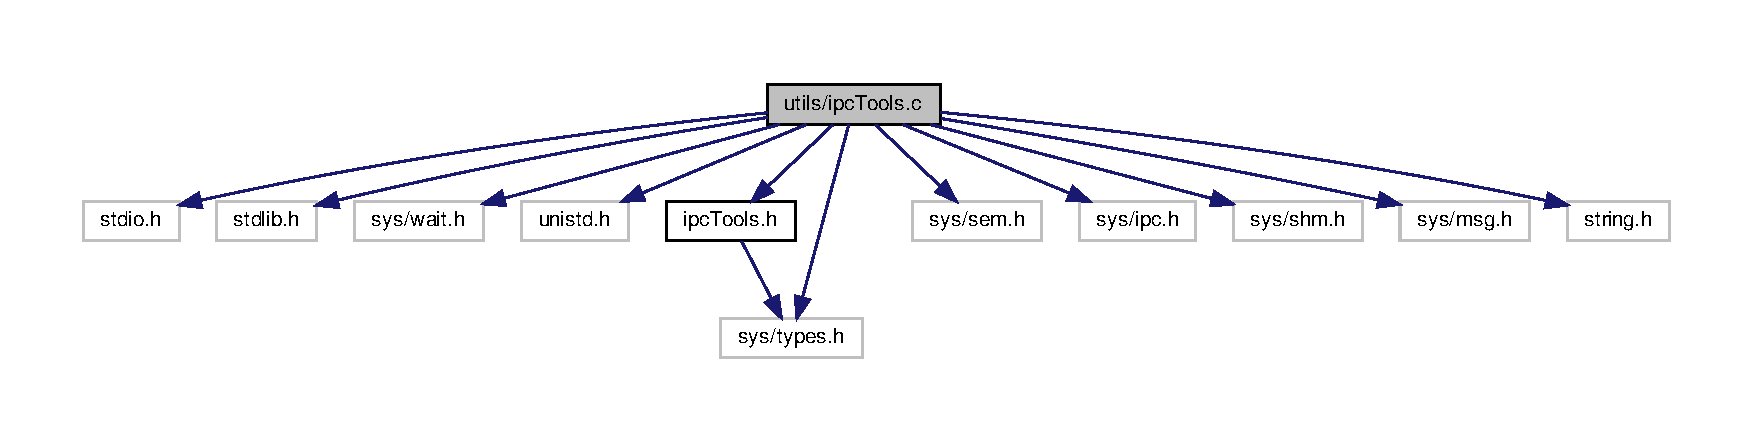
\includegraphics[width=350pt]{ipcTools_8c__incl}
\end{center}
\end{figure}
\subsection*{Macros}
\begin{DoxyCompactItemize}
\item 
\mbox{\Hypertarget{ipcTools_8c_a70ed59adcb4159ac551058053e649640}\label{ipcTools_8c_a70ed59adcb4159ac551058053e649640}} 
\#define {\bfseries S\+I\+ZE}~1024
\end{DoxyCompactItemize}
\subsection*{Functions}
\begin{DoxyCompactItemize}
\item 
int \hyperlink{ipcTools_8c_a45c8a1cc742b770f79825e79aa0c8ce7}{semalloc} (key\+\_\+t key, int val\+Init)
\begin{DoxyCompactList}\small\item\em This function create a semaphore. \end{DoxyCompactList}\item 
void \hyperlink{ipcTools_8c_a07d9975feec68c95cb5aba62b9d24ed8}{P} (int semid)
\begin{DoxyCompactList}\small\item\em This function increments the value of the semaphore. \end{DoxyCompactList}\item 
void \hyperlink{ipcTools_8c_a8a7b1645beb620891b3a8256143791e4}{V} (int semid)
\begin{DoxyCompactList}\small\item\em This function decrements the semaphore value. \end{DoxyCompactList}\item 
int \hyperlink{ipcTools_8c_a1a1666796045a3210edd37d16b0f9625}{semfree} (int semid)
\begin{DoxyCompactList}\small\item\em This function destroy the semaphore. \end{DoxyCompactList}\item 
int \hyperlink{ipcTools_8c_a88d7899467093e27a485527986aad253}{mutalloc} (key\+\_\+t key)
\begin{DoxyCompactList}\small\item\em This function allocate a Mutex. \end{DoxyCompactList}\item 
int \hyperlink{ipcTools_8c_a518dd2f4cfca662050363c790fb88972}{mutfree} (int semid)
\begin{DoxyCompactList}\small\item\em this function desallocate a Mutex \end{DoxyCompactList}\item 
\mbox{\Hypertarget{ipcTools_8c_aaae3779ba3c90a6bd1db639fd20ef251}\label{ipcTools_8c_aaae3779ba3c90a6bd1db639fd20ef251}} 
void $\ast$ {\bfseries shmalloc} (key\+\_\+t key, int size)
\item 
\mbox{\Hypertarget{ipcTools_8c_af6b34b8a7db92f7b60d335e3f06b8e34}\label{ipcTools_8c_af6b34b8a7db92f7b60d335e3f06b8e34}} 
int {\bfseries shmfree} (key\+\_\+t key)
\item 
\mbox{\Hypertarget{ipcTools_8c_abada598767ab7be4c217842b75d7fdf7}\label{ipcTools_8c_abada598767ab7be4c217842b75d7fdf7}} 
int {\bfseries msgalloc} (key\+\_\+t key)
\item 
\mbox{\Hypertarget{ipcTools_8c_a9bbc811831f58b58ba8af20811b114c8}\label{ipcTools_8c_a9bbc811831f58b58ba8af20811b114c8}} 
int {\bfseries msgfree} (int msgqid)
\item 
\mbox{\Hypertarget{ipcTools_8c_a531a39a4d3ac97936b502754c60cd79d}\label{ipcTools_8c_a531a39a4d3ac97936b502754c60cd79d}} 
int {\bfseries msgsend} (int msqid, char $\ast$msg, int msg\+Size)
\item 
\mbox{\Hypertarget{ipcTools_8c_a8e88811e1c78a08223e666537e5d0aac}\label{ipcTools_8c_a8e88811e1c78a08223e666537e5d0aac}} 
int {\bfseries msgrecv} (int msqid, char $\ast$msg, int msg\+Size)
\end{DoxyCompactItemize}


\subsection{Detailed Description}
This file helps to manage icp Semaphores and mutex. 

\begin{DoxyAuthor}{Author}
Nicolas C\+I\+B\+U\+L\+KA -\/ Kevin B\+E\+R\+N\+A\+RD -\/ Aelien M\+O\+U\+B\+E\+C\+HE 
\end{DoxyAuthor}
\begin{DoxyVersion}{Version}
0.\+1 
\end{DoxyVersion}
\begin{DoxyDate}{Date}
2021-\/03-\/15
\end{DoxyDate}
\begin{DoxyCopyright}{Copyright}
Copyright (c) 2021 
\end{DoxyCopyright}


\subsection{Function Documentation}
\mbox{\Hypertarget{ipcTools_8c_a88d7899467093e27a485527986aad253}\label{ipcTools_8c_a88d7899467093e27a485527986aad253}} 
\index{ipc\+Tools.\+c@{ipc\+Tools.\+c}!mutalloc@{mutalloc}}
\index{mutalloc@{mutalloc}!ipc\+Tools.\+c@{ipc\+Tools.\+c}}
\subsubsection{\texorpdfstring{mutalloc()}{mutalloc()}}
{\footnotesize\ttfamily int mutalloc (\begin{DoxyParamCaption}\item[{key\+\_\+t}]{key }\end{DoxyParamCaption})}



This function allocate a Mutex. 


\begin{DoxyParams}{Parameters}
{\em key} & a key\+\_\+t variable to guarantee the unicity of the mutex \\
\hline
\end{DoxyParams}
\begin{DoxyReturn}{Returns}
An Integer which is the mutex identifier 
\end{DoxyReturn}
\mbox{\Hypertarget{ipcTools_8c_a518dd2f4cfca662050363c790fb88972}\label{ipcTools_8c_a518dd2f4cfca662050363c790fb88972}} 
\index{ipc\+Tools.\+c@{ipc\+Tools.\+c}!mutfree@{mutfree}}
\index{mutfree@{mutfree}!ipc\+Tools.\+c@{ipc\+Tools.\+c}}
\subsubsection{\texorpdfstring{mutfree()}{mutfree()}}
{\footnotesize\ttfamily int mutfree (\begin{DoxyParamCaption}\item[{int}]{semid }\end{DoxyParamCaption})}



this function desallocate a Mutex 


\begin{DoxyParams}{Parameters}
{\em semid} & The identifier of the Mutex \\
\hline
\end{DoxyParams}
\begin{DoxyReturn}{Returns}
An Integer with the value -\/1 if an error occured, 0 if not 
\end{DoxyReturn}
\mbox{\Hypertarget{ipcTools_8c_a07d9975feec68c95cb5aba62b9d24ed8}\label{ipcTools_8c_a07d9975feec68c95cb5aba62b9d24ed8}} 
\index{ipc\+Tools.\+c@{ipc\+Tools.\+c}!P@{P}}
\index{P@{P}!ipc\+Tools.\+c@{ipc\+Tools.\+c}}
\subsubsection{\texorpdfstring{P()}{P()}}
{\footnotesize\ttfamily void P (\begin{DoxyParamCaption}\item[{int}]{semid }\end{DoxyParamCaption})}



This function increments the value of the semaphore. 


\begin{DoxyParams}{Parameters}
{\em semid} & The Identifier of the Semaphore \\
\hline
\end{DoxyParams}
\mbox{\Hypertarget{ipcTools_8c_a45c8a1cc742b770f79825e79aa0c8ce7}\label{ipcTools_8c_a45c8a1cc742b770f79825e79aa0c8ce7}} 
\index{ipc\+Tools.\+c@{ipc\+Tools.\+c}!semalloc@{semalloc}}
\index{semalloc@{semalloc}!ipc\+Tools.\+c@{ipc\+Tools.\+c}}
\subsubsection{\texorpdfstring{semalloc()}{semalloc()}}
{\footnotesize\ttfamily int semalloc (\begin{DoxyParamCaption}\item[{key\+\_\+t}]{key,  }\item[{int}]{val\+Init }\end{DoxyParamCaption})}



This function create a semaphore. 


\begin{DoxyParams}{Parameters}
{\em key} & A key to guarantee the unicity of the Semaphore \\
\hline
{\em val\+Init} & The value that will contains the semaphore when it will be initialise \\
\hline
\end{DoxyParams}
\begin{DoxyReturn}{Returns}
an Integer that will be the semaphore identifier 
\end{DoxyReturn}
\mbox{\Hypertarget{ipcTools_8c_a1a1666796045a3210edd37d16b0f9625}\label{ipcTools_8c_a1a1666796045a3210edd37d16b0f9625}} 
\index{ipc\+Tools.\+c@{ipc\+Tools.\+c}!semfree@{semfree}}
\index{semfree@{semfree}!ipc\+Tools.\+c@{ipc\+Tools.\+c}}
\subsubsection{\texorpdfstring{semfree()}{semfree()}}
{\footnotesize\ttfamily int semfree (\begin{DoxyParamCaption}\item[{int}]{semid }\end{DoxyParamCaption})}



This function destroy the semaphore. 


\begin{DoxyParams}{Parameters}
{\em semid} & The identifier of the semaphore \\
\hline
\end{DoxyParams}
\begin{DoxyReturn}{Returns}
an Integer with the value -\/1 if a problem occured, 0 if not 
\end{DoxyReturn}
\mbox{\Hypertarget{ipcTools_8c_a8a7b1645beb620891b3a8256143791e4}\label{ipcTools_8c_a8a7b1645beb620891b3a8256143791e4}} 
\index{ipc\+Tools.\+c@{ipc\+Tools.\+c}!V@{V}}
\index{V@{V}!ipc\+Tools.\+c@{ipc\+Tools.\+c}}
\subsubsection{\texorpdfstring{V()}{V()}}
{\footnotesize\ttfamily void V (\begin{DoxyParamCaption}\item[{int}]{semid }\end{DoxyParamCaption})}



This function decrements the semaphore value. 


\begin{DoxyParams}{Parameters}
{\em semid} & The indentifier of the semaphore \\
\hline
\end{DoxyParams}

\hypertarget{memory_8c}{}\section{utils/memory.c File Reference}
\label{memory_8c}\index{utils/memory.\+c@{utils/memory.\+c}}


This file is the .c that allow to do all the operations of allocation/free on the memory.  


{\ttfamily \#include $<$stdio.\+h$>$}\newline
{\ttfamily \#include $<$unistd.\+h$>$}\newline
{\ttfamily \#include $<$stdlib.\+h$>$}\newline
{\ttfamily \#include $<$sys/types.\+h$>$}\newline
{\ttfamily \#include $<$sys/ipc.\+h$>$}\newline
{\ttfamily \#include \char`\"{}memory.\+h\char`\"{}}\newline
{\ttfamily \#include \char`\"{}ipc\+Tools.\+h\char`\"{}}\newline
Include dependency graph for memory.\+c\+:
\nopagebreak
\begin{figure}[H]
\begin{center}
\leavevmode
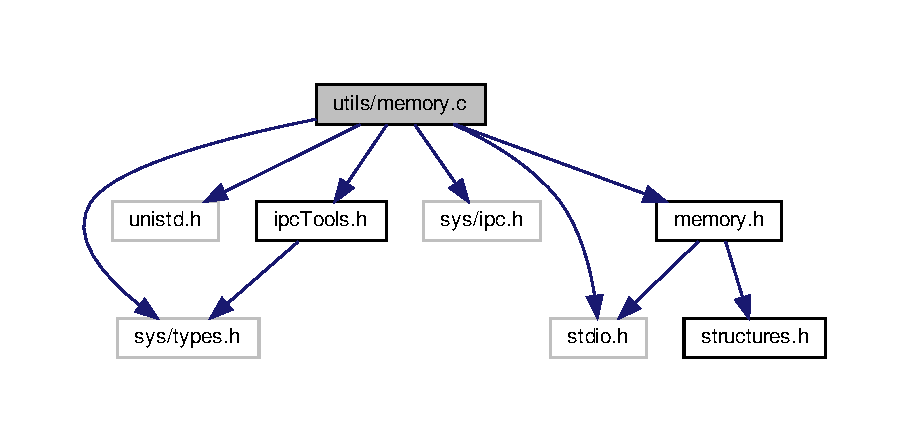
\includegraphics[width=350pt]{memory_8c__incl}
\end{center}
\end{figure}
\subsection*{Functions}
\begin{DoxyCompactItemize}
\item 
int \hyperlink{memory_8c_a10ddc18ec8b4edd1c9d5a0c2ebb71cda}{init\+Memory} (int size)
\begin{DoxyCompactList}\small\item\em Function to initiate the memory list. \end{DoxyCompactList}\item 
int \hyperlink{memory_8c_a8d862dc01c44bfabc8d952bb77f8da89}{free\+Memory} ()
\begin{DoxyCompactList}\small\item\em This function will free the great \hyperlink{structMemory}{Memory} structure. \end{DoxyCompactList}\item 
void $\ast$ \hyperlink{memory_8c_ad2337efa36c02f3d7e198fd2154a2d6a}{my\+Alloc} (int size)
\begin{DoxyCompactList}\small\item\em This function will do the allocation of a block, according to the size given in parameter. \end{DoxyCompactList}\item 
int \hyperlink{memory_8c_aeedb1fea6edab8d3c622675777ccd312}{my\+Free} (void $\ast$p)
\begin{DoxyCompactList}\small\item\em The Function that free the memory area given in parameter. \end{DoxyCompactList}\item 
\hyperlink{structPaginationUnit}{Pagination\+Unit} $\ast$ \hyperlink{memory_8c_aba9b1a029767f29ea614baff4aa1d6a9}{get\+First\+Pagination\+Unit} ()
\begin{DoxyCompactList}\small\item\em Get the adress of the First free Pagination Unit. \end{DoxyCompactList}\item 
void $\ast$ \hyperlink{memory_8c_a053ccff0042bef6fb33d55231236bbe9}{get\+Best\+Fit} (int size)
\begin{DoxyCompactList}\small\item\em Get the adress of the first element of the data\+Array that would have enough place after This according to the best Fit Algorithm. \end{DoxyCompactList}\item 
void \hyperlink{memory_8c_abc38fc84b1593301b41e5d411500814e}{actualize\+Allocated\+Map} (int start\+Pos, int size)
\begin{DoxyCompactList}\small\item\em This function will update the map of allocated\+Adress, to help best\+Fit Algorithm later. This will turn all the elements in the aimed area in 1 to say that those elements are allocoated. \end{DoxyCompactList}\item 
void \hyperlink{memory_8c_a778926f90d7c9d349798358e05c10e90}{reset\+Allocated\+Map} (int start\+Pos, int size)
\begin{DoxyCompactList}\small\item\em This function will update the map of allocated\+Adress, to help best\+Fit Algorithm later. This will turn all the elements in the aimed area in 0 to say that those elements are now released. \end{DoxyCompactList}\end{DoxyCompactItemize}
\subsection*{Variables}
\begin{DoxyCompactItemize}
\item 
\mbox{\Hypertarget{memory_8c_a710310e3d93bcc274cec2872f69527b9}\label{memory_8c_a710310e3d93bcc274cec2872f69527b9}} 
\hyperlink{structMemory}{Memory} \hyperlink{memory_8c_a710310e3d93bcc274cec2872f69527b9}{memory}
\begin{DoxyCompactList}\small\item\em The memory variable that will store all the allocated elements. \end{DoxyCompactList}\end{DoxyCompactItemize}


\subsection{Detailed Description}
This file is the .c that allow to do all the operations of allocation/free on the memory. 

\begin{DoxyAuthor}{Author}
Nicolas C\+I\+B\+U\+L\+KA -\/ Kevin B\+E\+R\+N\+A\+RD -\/ Aelien M\+O\+U\+B\+E\+C\+HE 
\end{DoxyAuthor}
\begin{DoxyVersion}{Version}
0.\+1 
\end{DoxyVersion}
\begin{DoxyDate}{Date}
2021-\/03-\/14
\end{DoxyDate}
\begin{DoxyCopyright}{Copyright}
Copyright (c) 2021 
\end{DoxyCopyright}


\subsection{Function Documentation}
\mbox{\Hypertarget{memory_8c_abc38fc84b1593301b41e5d411500814e}\label{memory_8c_abc38fc84b1593301b41e5d411500814e}} 
\index{memory.\+c@{memory.\+c}!actualize\+Allocated\+Map@{actualize\+Allocated\+Map}}
\index{actualize\+Allocated\+Map@{actualize\+Allocated\+Map}!memory.\+c@{memory.\+c}}
\subsubsection{\texorpdfstring{actualize\+Allocated\+Map()}{actualizeAllocatedMap()}}
{\footnotesize\ttfamily void actualize\+Allocated\+Map (\begin{DoxyParamCaption}\item[{int}]{start\+Pos,  }\item[{int}]{size }\end{DoxyParamCaption})}



This function will update the map of allocated\+Adress, to help best\+Fit Algorithm later. This will turn all the elements in the aimed area in 1 to say that those elements are allocoated. 


\begin{DoxyParams}{Parameters}
{\em start\+Pos} & \+: the starting position of the allocated area \\
\hline
{\em size} & \+: the size of the allocated area \\
\hline
\end{DoxyParams}
\mbox{\Hypertarget{memory_8c_a8d862dc01c44bfabc8d952bb77f8da89}\label{memory_8c_a8d862dc01c44bfabc8d952bb77f8da89}} 
\index{memory.\+c@{memory.\+c}!free\+Memory@{free\+Memory}}
\index{free\+Memory@{free\+Memory}!memory.\+c@{memory.\+c}}
\subsubsection{\texorpdfstring{free\+Memory()}{freeMemory()}}
{\footnotesize\ttfamily int free\+Memory (\begin{DoxyParamCaption}{ }\end{DoxyParamCaption})}



This function will free the great \hyperlink{structMemory}{Memory} structure. 

\begin{DoxyReturn}{Returns}
An Integer that wille be the size that the function has got back, or -\/1 if an error occured 
\end{DoxyReturn}
\mbox{\Hypertarget{memory_8c_a053ccff0042bef6fb33d55231236bbe9}\label{memory_8c_a053ccff0042bef6fb33d55231236bbe9}} 
\index{memory.\+c@{memory.\+c}!get\+Best\+Fit@{get\+Best\+Fit}}
\index{get\+Best\+Fit@{get\+Best\+Fit}!memory.\+c@{memory.\+c}}
\subsubsection{\texorpdfstring{get\+Best\+Fit()}{getBestFit()}}
{\footnotesize\ttfamily void$\ast$ get\+Best\+Fit (\begin{DoxyParamCaption}\item[{int}]{size }\end{DoxyParamCaption})}



Get the adress of the first element of the data\+Array that would have enough place after This according to the best Fit Algorithm. 


\begin{DoxyParams}{Parameters}
{\em size} & The needed size for the block \\
\hline
\end{DoxyParams}
\begin{DoxyReturn}{Returns}
void$\ast$ \+: The adress of the first element of the block 
\end{DoxyReturn}
\mbox{\Hypertarget{memory_8c_aba9b1a029767f29ea614baff4aa1d6a9}\label{memory_8c_aba9b1a029767f29ea614baff4aa1d6a9}} 
\index{memory.\+c@{memory.\+c}!get\+First\+Pagination\+Unit@{get\+First\+Pagination\+Unit}}
\index{get\+First\+Pagination\+Unit@{get\+First\+Pagination\+Unit}!memory.\+c@{memory.\+c}}
\subsubsection{\texorpdfstring{get\+First\+Pagination\+Unit()}{getFirstPaginationUnit()}}
{\footnotesize\ttfamily \hyperlink{structPaginationUnit}{Pagination\+Unit}$\ast$ get\+First\+Pagination\+Unit (\begin{DoxyParamCaption}{ }\end{DoxyParamCaption})}



Get the adress of the First free Pagination Unit. 

\begin{DoxyReturn}{Returns}
Pagination\+Unit$\ast$ 
\end{DoxyReturn}
\mbox{\Hypertarget{memory_8c_a10ddc18ec8b4edd1c9d5a0c2ebb71cda}\label{memory_8c_a10ddc18ec8b4edd1c9d5a0c2ebb71cda}} 
\index{memory.\+c@{memory.\+c}!init\+Memory@{init\+Memory}}
\index{init\+Memory@{init\+Memory}!memory.\+c@{memory.\+c}}
\subsubsection{\texorpdfstring{init\+Memory()}{initMemory()}}
{\footnotesize\ttfamily int init\+Memory (\begin{DoxyParamCaption}\item[{int}]{size }\end{DoxyParamCaption})}



Function to initiate the memory list. 


\begin{DoxyParams}{Parameters}
{\em n} & Represent the size of the great structure that will contains all the allocated elements \\
\hline
\end{DoxyParams}
\begin{DoxyReturn}{Returns}
An Integer that will be 0 if an error occured, or the size given in parameter if the operation succeed 
\end{DoxyReturn}
\mbox{\Hypertarget{memory_8c_ad2337efa36c02f3d7e198fd2154a2d6a}\label{memory_8c_ad2337efa36c02f3d7e198fd2154a2d6a}} 
\index{memory.\+c@{memory.\+c}!my\+Alloc@{my\+Alloc}}
\index{my\+Alloc@{my\+Alloc}!memory.\+c@{memory.\+c}}
\subsubsection{\texorpdfstring{my\+Alloc()}{myAlloc()}}
{\footnotesize\ttfamily void$\ast$ my\+Alloc (\begin{DoxyParamCaption}\item[{int}]{size }\end{DoxyParamCaption})}



This function will do the allocation of a block, according to the size given in parameter. 


\begin{DoxyParams}{Parameters}
{\em size} & The size of the data block we want \\
\hline
\end{DoxyParams}
\begin{DoxyReturn}{Returns}
A void$\ast$ which is the adress of the data block 
\end{DoxyReturn}
\mbox{\Hypertarget{memory_8c_aeedb1fea6edab8d3c622675777ccd312}\label{memory_8c_aeedb1fea6edab8d3c622675777ccd312}} 
\index{memory.\+c@{memory.\+c}!my\+Free@{my\+Free}}
\index{my\+Free@{my\+Free}!memory.\+c@{memory.\+c}}
\subsubsection{\texorpdfstring{my\+Free()}{myFree()}}
{\footnotesize\ttfamily int my\+Free (\begin{DoxyParamCaption}\item[{void $\ast$}]{p }\end{DoxyParamCaption})}



The Function that free the memory area given in parameter. 


\begin{DoxyParams}{Parameters}
{\em p} & The pointer to the data block \\
\hline
\end{DoxyParams}
\begin{DoxyReturn}{Returns}
an Integer the size of the memory removed 
\end{DoxyReturn}
\mbox{\Hypertarget{memory_8c_a778926f90d7c9d349798358e05c10e90}\label{memory_8c_a778926f90d7c9d349798358e05c10e90}} 
\index{memory.\+c@{memory.\+c}!reset\+Allocated\+Map@{reset\+Allocated\+Map}}
\index{reset\+Allocated\+Map@{reset\+Allocated\+Map}!memory.\+c@{memory.\+c}}
\subsubsection{\texorpdfstring{reset\+Allocated\+Map()}{resetAllocatedMap()}}
{\footnotesize\ttfamily void reset\+Allocated\+Map (\begin{DoxyParamCaption}\item[{int}]{start\+Pos,  }\item[{int}]{size }\end{DoxyParamCaption})}



This function will update the map of allocated\+Adress, to help best\+Fit Algorithm later. This will turn all the elements in the aimed area in 0 to say that those elements are now released. 


\begin{DoxyParams}{Parameters}
{\em start\+Pos} & \+: the starting position of the allocated area \\
\hline
{\em size} & \+: the size of the allocated area \\
\hline
\end{DoxyParams}

\hypertarget{structures_8c}{}\section{utils/structures.c File Reference}
\label{structures_8c}\index{utils/structures.\+c@{utils/structures.\+c}}


this file is the .c used to manipulate the header block  


{\ttfamily \#include $<$stdio.\+h$>$}\newline
{\ttfamily \#include $<$stdlib.\+h$>$}\newline
{\ttfamily \#include \char`\"{}structures.\+h\char`\"{}}\newline
{\ttfamily \#include \char`\"{}ipc\+Tools.\+h\char`\"{}}\newline
Include dependency graph for structures.\+c\+:
\nopagebreak
\begin{figure}[H]
\begin{center}
\leavevmode
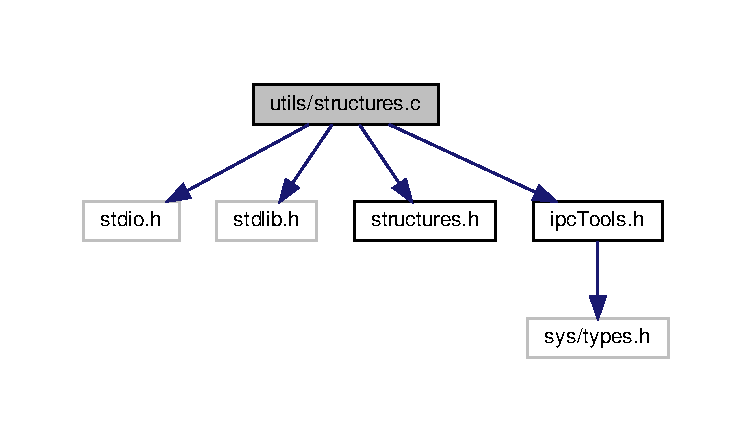
\includegraphics[width=350pt]{structures_8c__incl}
\end{center}
\end{figure}
\subsection*{Functions}
\begin{DoxyCompactItemize}
\item 
\hyperlink{structPaginationUnit}{Pagination\+Unit} \hyperlink{structures_8c_a12c11e0b78c302f5e32758f17422dc91}{init\+Pagination\+Unit} ()
\begin{DoxyCompactList}\small\item\em Initialise an empty \hyperlink{structPaginationUnit}{Pagination\+Unit}. \end{DoxyCompactList}\item 
void \hyperlink{structures_8c_afcf40202075d3f4ca3f13a4e1da22a9e}{reset\+Pagination\+Unit} (\hyperlink{structPaginationUnit}{Pagination\+Unit} $\ast$unit)
\begin{DoxyCompactList}\small\item\em reset a given pagination\+Unit \end{DoxyCompactList}\item 
\hyperlink{structDataRibbon}{Data\+Ribbon} \hyperlink{structures_8c_a259c0deed04105e9182970a82bab6940}{init\+Data\+Ribbon} (int size)
\begin{DoxyCompactList}\small\item\em Initialise the Data Ribbon that will contains all our values. \end{DoxyCompactList}\item 
void \hyperlink{structures_8c_a027000b01aec96c860c0a833bfe94355}{free\+Data\+Ribbon} (\hyperlink{structDataRibbon}{Data\+Ribbon} $\ast$ribbon)
\begin{DoxyCompactList}\small\item\em Free a given \hyperlink{structDataRibbon}{Data\+Ribbon}. \end{DoxyCompactList}\end{DoxyCompactItemize}


\subsection{Detailed Description}
this file is the .c used to manipulate the header block 

this file is the .h used to manipulate the pagination block

\begin{DoxyAuthor}{Author}
Nicolas C\+I\+B\+U\+L\+KA -\/ Kevin B\+E\+R\+N\+A\+RD -\/ Aelien M\+O\+U\+B\+E\+C\+HE 
\end{DoxyAuthor}
\begin{DoxyVersion}{Version}
0.\+1 
\end{DoxyVersion}
\begin{DoxyDate}{Date}
2021-\/03-\/14
\end{DoxyDate}
\begin{DoxyCopyright}{Copyright}
Copyright (c) 2021 
\end{DoxyCopyright}


\subsection{Function Documentation}
\mbox{\Hypertarget{structures_8c_a027000b01aec96c860c0a833bfe94355}\label{structures_8c_a027000b01aec96c860c0a833bfe94355}} 
\index{structures.\+c@{structures.\+c}!free\+Data\+Ribbon@{free\+Data\+Ribbon}}
\index{free\+Data\+Ribbon@{free\+Data\+Ribbon}!structures.\+c@{structures.\+c}}
\subsubsection{\texorpdfstring{free\+Data\+Ribbon()}{freeDataRibbon()}}
{\footnotesize\ttfamily void free\+Data\+Ribbon (\begin{DoxyParamCaption}\item[{\hyperlink{structDataRibbon}{Data\+Ribbon} $\ast$}]{ribbon }\end{DoxyParamCaption})}



Free a given \hyperlink{structDataRibbon}{Data\+Ribbon}. 


\begin{DoxyParams}{Parameters}
{\em ribbon} & \+: The Ribbon that will be released \\
\hline
\end{DoxyParams}
\mbox{\Hypertarget{structures_8c_a259c0deed04105e9182970a82bab6940}\label{structures_8c_a259c0deed04105e9182970a82bab6940}} 
\index{structures.\+c@{structures.\+c}!init\+Data\+Ribbon@{init\+Data\+Ribbon}}
\index{init\+Data\+Ribbon@{init\+Data\+Ribbon}!structures.\+c@{structures.\+c}}
\subsubsection{\texorpdfstring{init\+Data\+Ribbon()}{initDataRibbon()}}
{\footnotesize\ttfamily \hyperlink{structDataRibbon}{Data\+Ribbon} init\+Data\+Ribbon (\begin{DoxyParamCaption}\item[{int}]{size }\end{DoxyParamCaption})}



Initialise the Data Ribbon that will contains all our values. 


\begin{DoxyParams}{Parameters}
{\em size} & The size of the Ribbon \\
\hline
\end{DoxyParams}
\begin{DoxyReturn}{Returns}
\hyperlink{structDataRibbon}{Data\+Ribbon} \+: the array that will contains all our data 
\end{DoxyReturn}
\mbox{\Hypertarget{structures_8c_a12c11e0b78c302f5e32758f17422dc91}\label{structures_8c_a12c11e0b78c302f5e32758f17422dc91}} 
\index{structures.\+c@{structures.\+c}!init\+Pagination\+Unit@{init\+Pagination\+Unit}}
\index{init\+Pagination\+Unit@{init\+Pagination\+Unit}!structures.\+c@{structures.\+c}}
\subsubsection{\texorpdfstring{init\+Pagination\+Unit()}{initPaginationUnit()}}
{\footnotesize\ttfamily \hyperlink{structPaginationUnit}{Pagination\+Unit} init\+Pagination\+Unit (\begin{DoxyParamCaption}{ }\end{DoxyParamCaption})}



Initialise an empty \hyperlink{structPaginationUnit}{Pagination\+Unit}. 

\begin{DoxyReturn}{Returns}
\hyperlink{structPaginationUnit}{Pagination\+Unit} 
\end{DoxyReturn}
\mbox{\Hypertarget{structures_8c_afcf40202075d3f4ca3f13a4e1da22a9e}\label{structures_8c_afcf40202075d3f4ca3f13a4e1da22a9e}} 
\index{structures.\+c@{structures.\+c}!reset\+Pagination\+Unit@{reset\+Pagination\+Unit}}
\index{reset\+Pagination\+Unit@{reset\+Pagination\+Unit}!structures.\+c@{structures.\+c}}
\subsubsection{\texorpdfstring{reset\+Pagination\+Unit()}{resetPaginationUnit()}}
{\footnotesize\ttfamily void reset\+Pagination\+Unit (\begin{DoxyParamCaption}\item[{\hyperlink{structPaginationUnit}{Pagination\+Unit} $\ast$}]{unit }\end{DoxyParamCaption})}



reset a given pagination\+Unit 


\begin{DoxyParams}{Parameters}
{\em unit} & \+: T\+He unit that will be reset \\
\hline
\end{DoxyParams}

%--- End generated contents ---

% Index
\backmatter
\newpage
\phantomsection
\clearemptydoublepage
\addcontentsline{toc}{chapter}{Index}
\printindex

\end{document}
